% ---------------------------------------------------
\chapter{Function-Level Code Replication (FLCR)}
\label{chap:flcr}
% ---------------------------------------------------

\section{Overview}
Function-Level Code Replication (FLCR) divides a program into individually replicated functions.
Each function maintains one or more redundant copies within the same total redundancy capacity
as region-level replication. At runtime, each replica is validated, and all function calls are
redirected through a runtime indirection layer to a verified target.
This introduces runtime indirection at function boundaries while maintaining normal control flow
inside each function body once execution begins.

% ---------------------------------------------------
\section{Mechanism}
FLCR introduces runtime redirection at function boundaries through a coordinated set of metadata
structures and control components that manage validation, selection, and indirection.
During compilation, each function call—whether direct or indirect—is rewritten to pass through
an indirection layer that dynamically resolves the target at runtime.
This ensures that every control transfer passes through a verification-aware interface,
maintaining consistent access to valid targets.

\subsection{Static Metadata}
Static metadata defines the structure and integrity information for all function replicas.
It is generated in two stages: partially at compile time and completed at post-link time once
code layout and binary contents are finalized.

\begin{itemize}
  \item \textbf{Function Address Table:}
        Generated at compile time. Lists the base address of every function replica so the
        runtime can locate and identify each function.
  \item \textbf{Function Size Table:}
        Generated at post-link time. Records the exact compiled size of each function replica,
        enabling accurate boundary identification for hash computation.
  \item \textbf{Function Hash Table:}
        Generated at post-link time. Stores the precomputed hash for each function replica.
        During execution, the validator recomputes these hashes to confirm integrity.
\end{itemize}

\subsection{Runtime Dynamic Data}
Dynamic metadata represents the current runtime state of all protected functions and is
updated during initialization.

\begin{itemize}
  \item \textbf{Indirection Table (ITab):}
        A fixed-size array indexed by function identifier.
        Each entry contains a pointer to the currently validated target.
        ITab supports all \textbf{direct calls}, where the function index is statically known.
  \item \textbf{Indirection Map (IMap):}
        A binary-searchable map sorted by function address.
        It contains entries for \textbf{all protected functions}, associating each original
        function address with its validated target.
        The IMap supports \textbf{indirect calls} (via function pointers or callbacks)
        and serves as the central reference structure for runtime validation and lookup.
        Its sorted layout allows deterministic binary search without dynamic allocation or hashing.
\end{itemize}

\subsection{Core Components}
\begin{itemize}
  \item \textbf{Validator:}
        Computes the hash for each function replica using the Function Address, Size, and Hash tables.
        Marks replicas as valid if the computed hash matches the expected reference value.

  \item \textbf{Selector:}
        Invokes the Validator to verify all function replicas and determine valid targets.
        If no valid replica exists, the Selector falls back to the first replica in the set.

  \item \textbf{Metadata Initializer:}
        Calls the Selector at startup and uses its results to populate all runtime dynamic structures.
        It writes the validated targets into ITab and IMap, initializes validation states,
        and finalizes all data structures for runtime access.

  \item \textbf{Indirect Resolver:}
        Executes only at \textbf{call sites that were originally indirect}, such as function pointers
        or callbacks. It searches the IMap for the entry corresponding to the original function
        address and retrieves the validated target before control transfer.
\end{itemize}

\subsection{Call-Site Transformation}
FLCR rewrites every function invocation to pass through an indirection layer that resolves
the callee to a validated target at runtime.
Two transformations are applied depending on whether the original call target is static or dynamic.

\begin{table}[h!]
  \centering
  \renewcommand{\arraystretch}{1.2}
  \begin{tabularx}{\linewidth}{|l|X|X|}
    \hline
    \textbf{Call Type} & \textbf{Original} & \textbf{Transformed} \\ \hline
    Direct call   & \texttt{call foo()} & \texttt{target ← ITab[FID\_foo]} → \texttt{call target()} \\ \hline
    Indirect call & \texttt{fptr()}     & \texttt{target ← resolver(fptr)} → \texttt{call target()} \\ \hline
  \end{tabularx}
  \caption{FLCR call-site transformation for direct and indirect calls.}
  \label{tab:flcr-callsite}
\end{table}

\textbf{Description:}
\begin{itemize}
  \item \textbf{Direct calls:}
        Each static call site is assigned a compile-time function identifier (FID).
        At runtime, the call retrieves its validated target from the Indirection Table (ITab)
        before execution.
  \item \textbf{Indirect calls:}
        Calls made through function pointers or callbacks are passed to the \textit{resolver},
        which performs a binary search on the Indirection Map (IMap) to locate the validated
        target corresponding to the original function address.
\end{itemize}

All function invocations—direct or indirect—therefore pass through the same validation-aware
indirection layer, ensuring that execution always targets verified code.

% ---------------------------------------------------
\section{Execution Flow}
At runtime, control first reaches the internal entry point \texttt{\_Entry}, which immediately
invokes the \textbf{Metadata Initializer} before transferring control to the validated
program entry replica (\texttt{Entry.1}).
The initializer calls the \textbf{Selector}, which in turn invokes the \textbf{Validator}
to verify all function replicas and identify valid targets.
Once validation is complete, the runtime indirection structures (\texttt{ITab} and
\texttt{IMap}) are populated so that subsequent execution proceeds entirely through
verified targets.

Figure~\ref{fig:baseline-sequence} shows a baseline execution sequence without replication,
where function calls occur as intended.
Figure~\ref{fig:flcr-sequence} illustrates the FLCR sequence,
where \texttt{\_Entry} and the \textbf{Metadata Initializer} together form a
startup trampoline that redirects control to the validated entry target.

\begin{enumerate}
  \item \textbf{\_Entry:} The trampoline entry point that calls the
        \textbf{Metadata Initializer} and then jumps to the validated \texttt{Entry.1} target.
  \item \textbf{Metadata Initialization:} Invokes the \textbf{Selector}, which calls the
        \textbf{Validator} to compute hashes and determine valid replicas for each function.
  \item \textbf{Runtime Structure Setup:} The Selector provides validated targets to the
        \textbf{Metadata Initializer}, which writes them into \texttt{ITab} and \texttt{IMap},
        finalizing the runtime data structures.
  \item \textbf{Entry.1 (Validated Entry):} Normal execution begins from the validated
        entry function. Direct calls fetch targets from \texttt{ITab};
        indirect calls use the \textbf{resolver} to look up targets in \texttt{IMap}.
\end{enumerate}

This startup sequence ensures that every function call—direct or indirect—is routed through
validated metadata and that all control-flow transitions occur within verified code regions.

\begin{figure}[t]
  \centering
  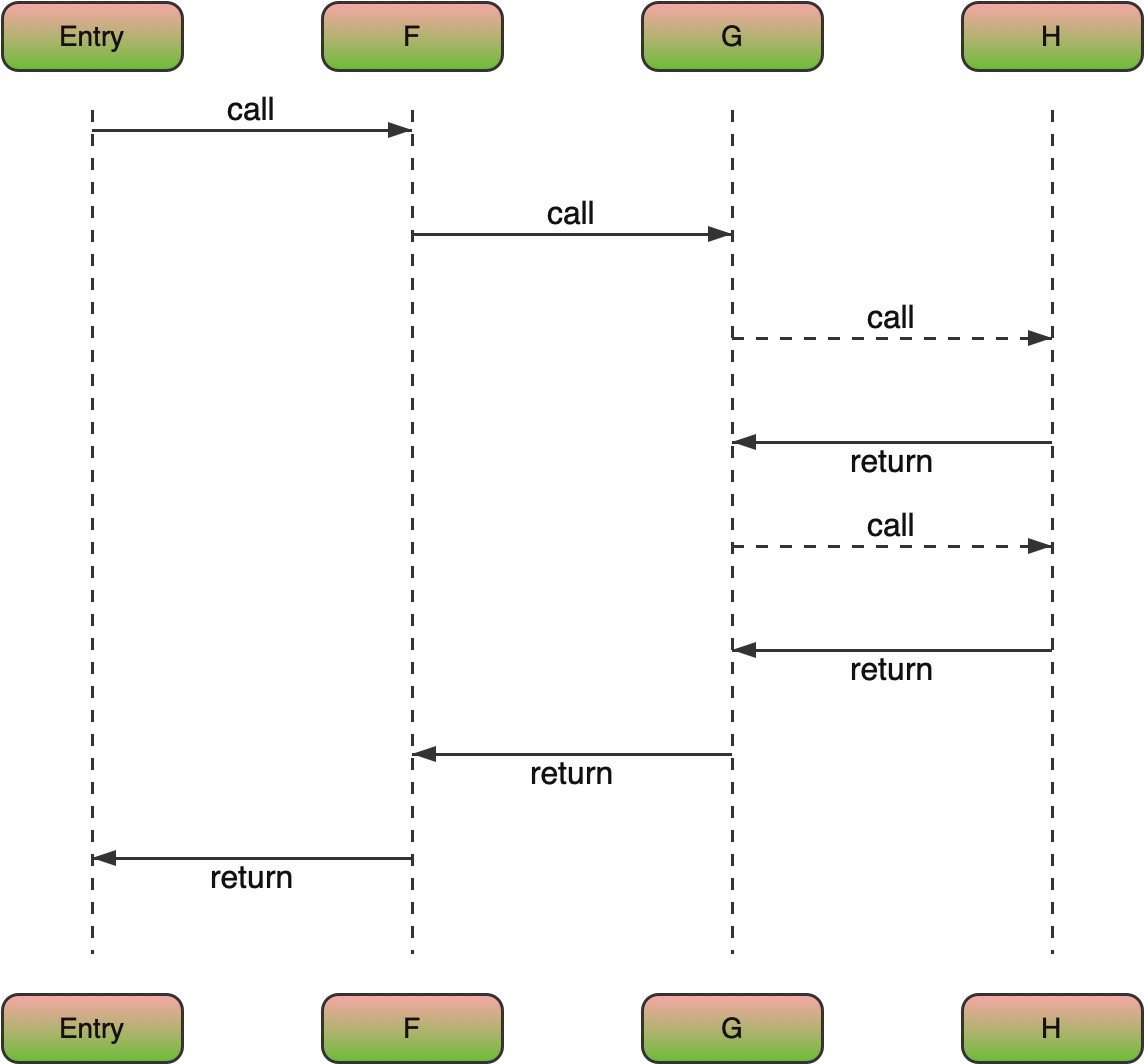
\includegraphics[width=0.9\linewidth]{Chapter-7/figs/baseline-sequence.png}
  \caption{Baseline execution sequence without replication or indirection.
           Function calls occur directly between functions without validation.}
  \label{fig:baseline-sequence}
\end{figure}

\begin{figure}[t]
  \centering
  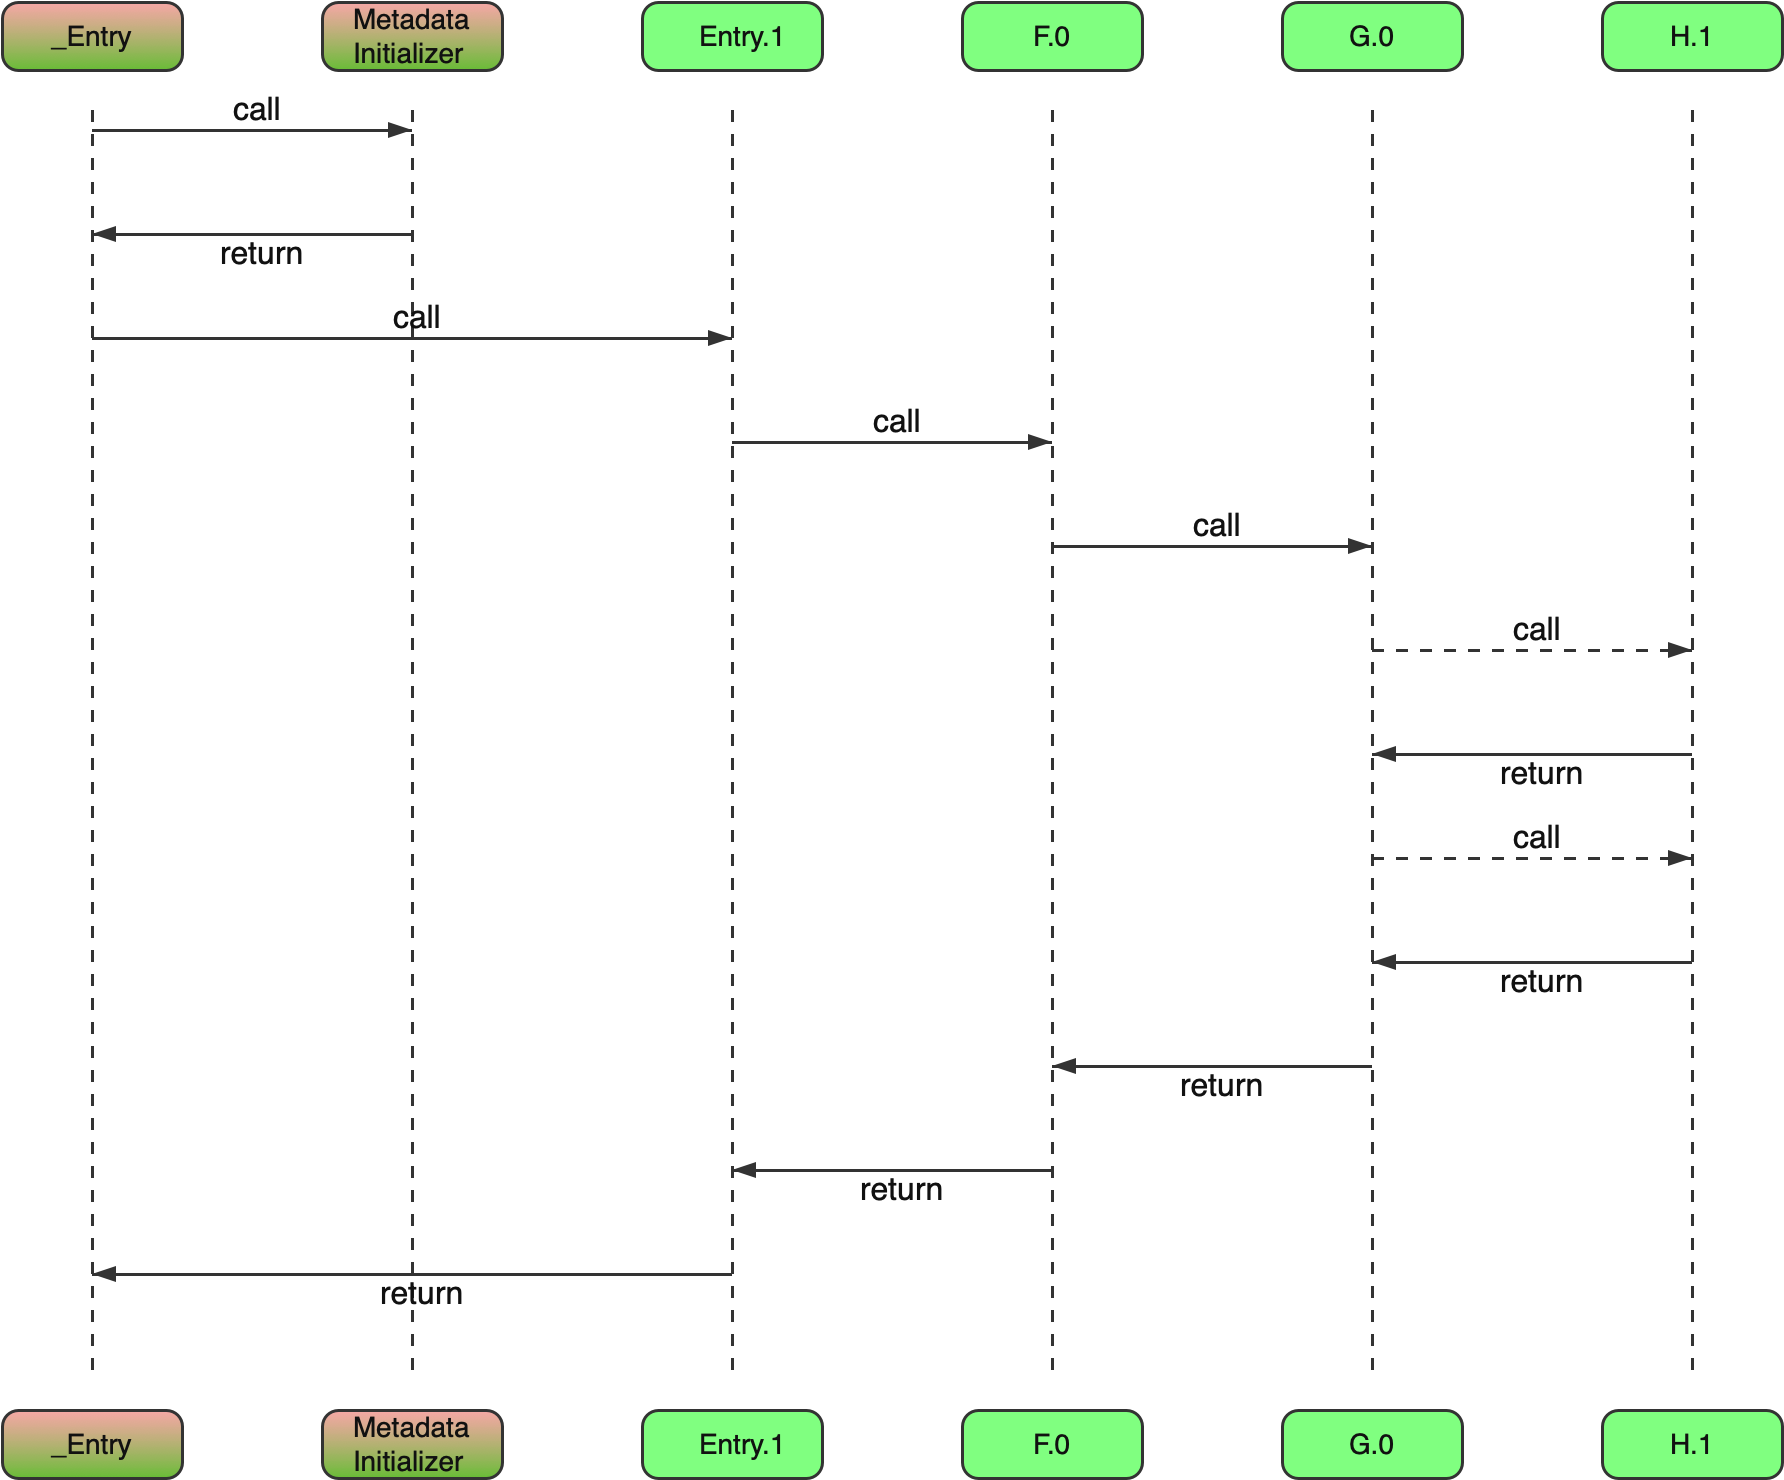
\includegraphics[width=0.9\linewidth]{Chapter-7/figs/flcr-sequence.png}
  \caption{Execution flow under FLCR. The internal \texttt{\_Entry} invokes the
           \textbf{Metadata Initializer}, which calls the \textbf{Selector} to validate and
           populate runtime structures. Control then transfers to the validated
           \texttt{Entry.1} target, after which all calls proceed through validated indirection.}
  \label{fig:flcr-sequence}
\end{figure}

% ---------------------------------------------------
\section{Limit Study}
The following limit study evaluates Function-Level Code Replication (FLCR) under controlled
fault injection to determine its reliability across a range of redundancy configurations.
This study uses the same experimental framework and methodology established for the
baseline and region-level replication (RLCR) analyses.

\subsection{Setup}
Each benchmark is configured to use the same total amount of redundant storage as in
the region-level experiments, but the replicas are distributed across individual functions
rather than entire code regions.
The fault injection method follows the same procedure as the baseline:
random bit flips are introduced directly into the program image while excluding shared
library functions and read-only data sections (\texttt{.data} and \texttt{.rodata}).
All injected faults are constrained to user-level executable regions to isolate the
impact of code corruption.

Each experiment executes 1,000 randomized trials per fault rate.
The primary metric measured is:
\begin{itemize}
  \item \textbf{Reliability:} The probability that all required functions execute
        correctly under a given fault density, measured as the fraction of successful
        program runs.
\end{itemize}

Figure~\ref{fig:flcr-reliability} summarizes observed reliability across fault densities
and compares FLCR with the unprotected baseline and RLCR configurations.

\begin{figure}[t]
  \centering
  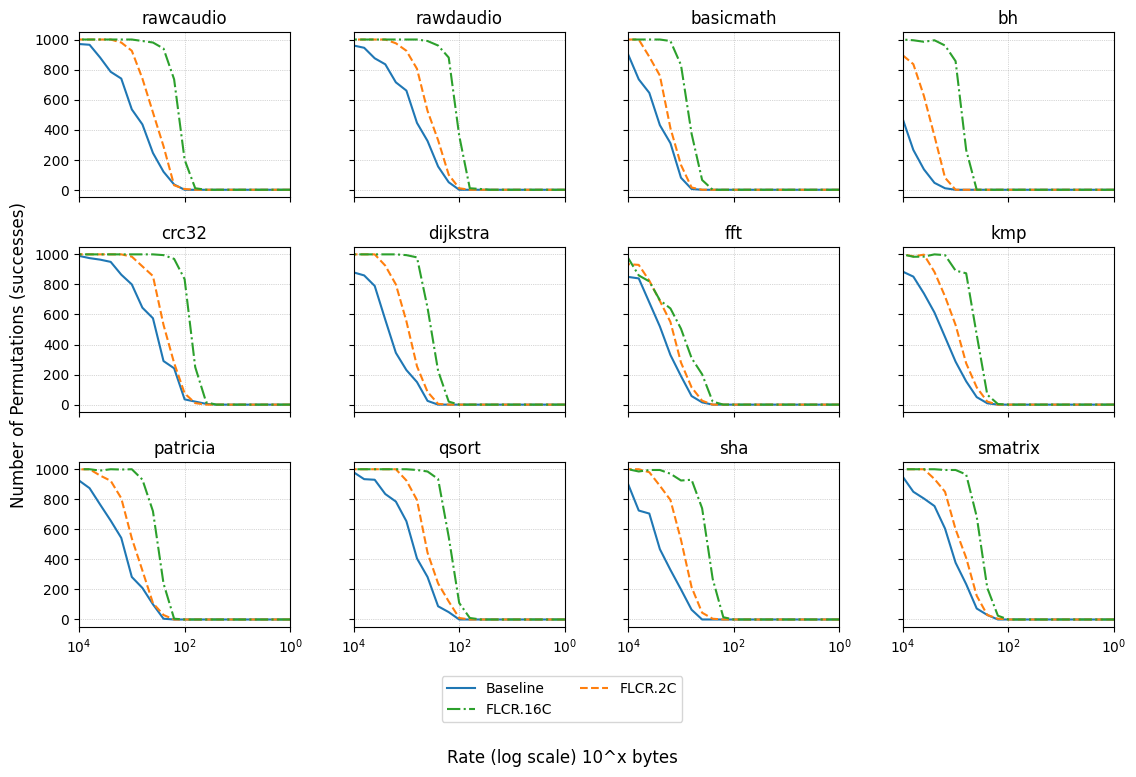
\includegraphics[width=\linewidth]{Chapter-7/figs/flcr-reliability.png}
  \caption{Reliability of FLCR under increasing fault density compared with baseline
           and RLCR configurations. Each curve represents the fraction of successful
           runs out of 1,000 trials.}
  \label{fig:flcr-reliability}
\end{figure}

\subsection{Results}
FLCR maintains correct execution in cases where region-level replication fails due to
localized corruption. Because each function is independently validated and redirected
through a verified target, faults that affect a single function do not compromise the
entire image. Reliability degrades gradually as fault density increases, reflecting
the probability that all required functions retain at least one valid replica.

\subsection{Interpretation}
These results confirm that distributing redundancy at the function level increases
fault containment and improves overall reliability under equal redundancy capacity.
Where RLCR invalidates an entire region after a single failure, FLCR isolates damage
to individual functions, preserving operational integrity of the remaining code.

The magnitude of improvement varies with the program’s function-size profile.
Benchmarks with many small functions benefit most, since localized faults are unlikely to
simultaneously eliminate all replicas of every required function. Conversely, workloads
dominated by a few large functions exhibit sharper reliability drop-offs because a single
faulted hot function removes a larger fraction of the effective code base.

\begin{figure}[t]
  \centering
  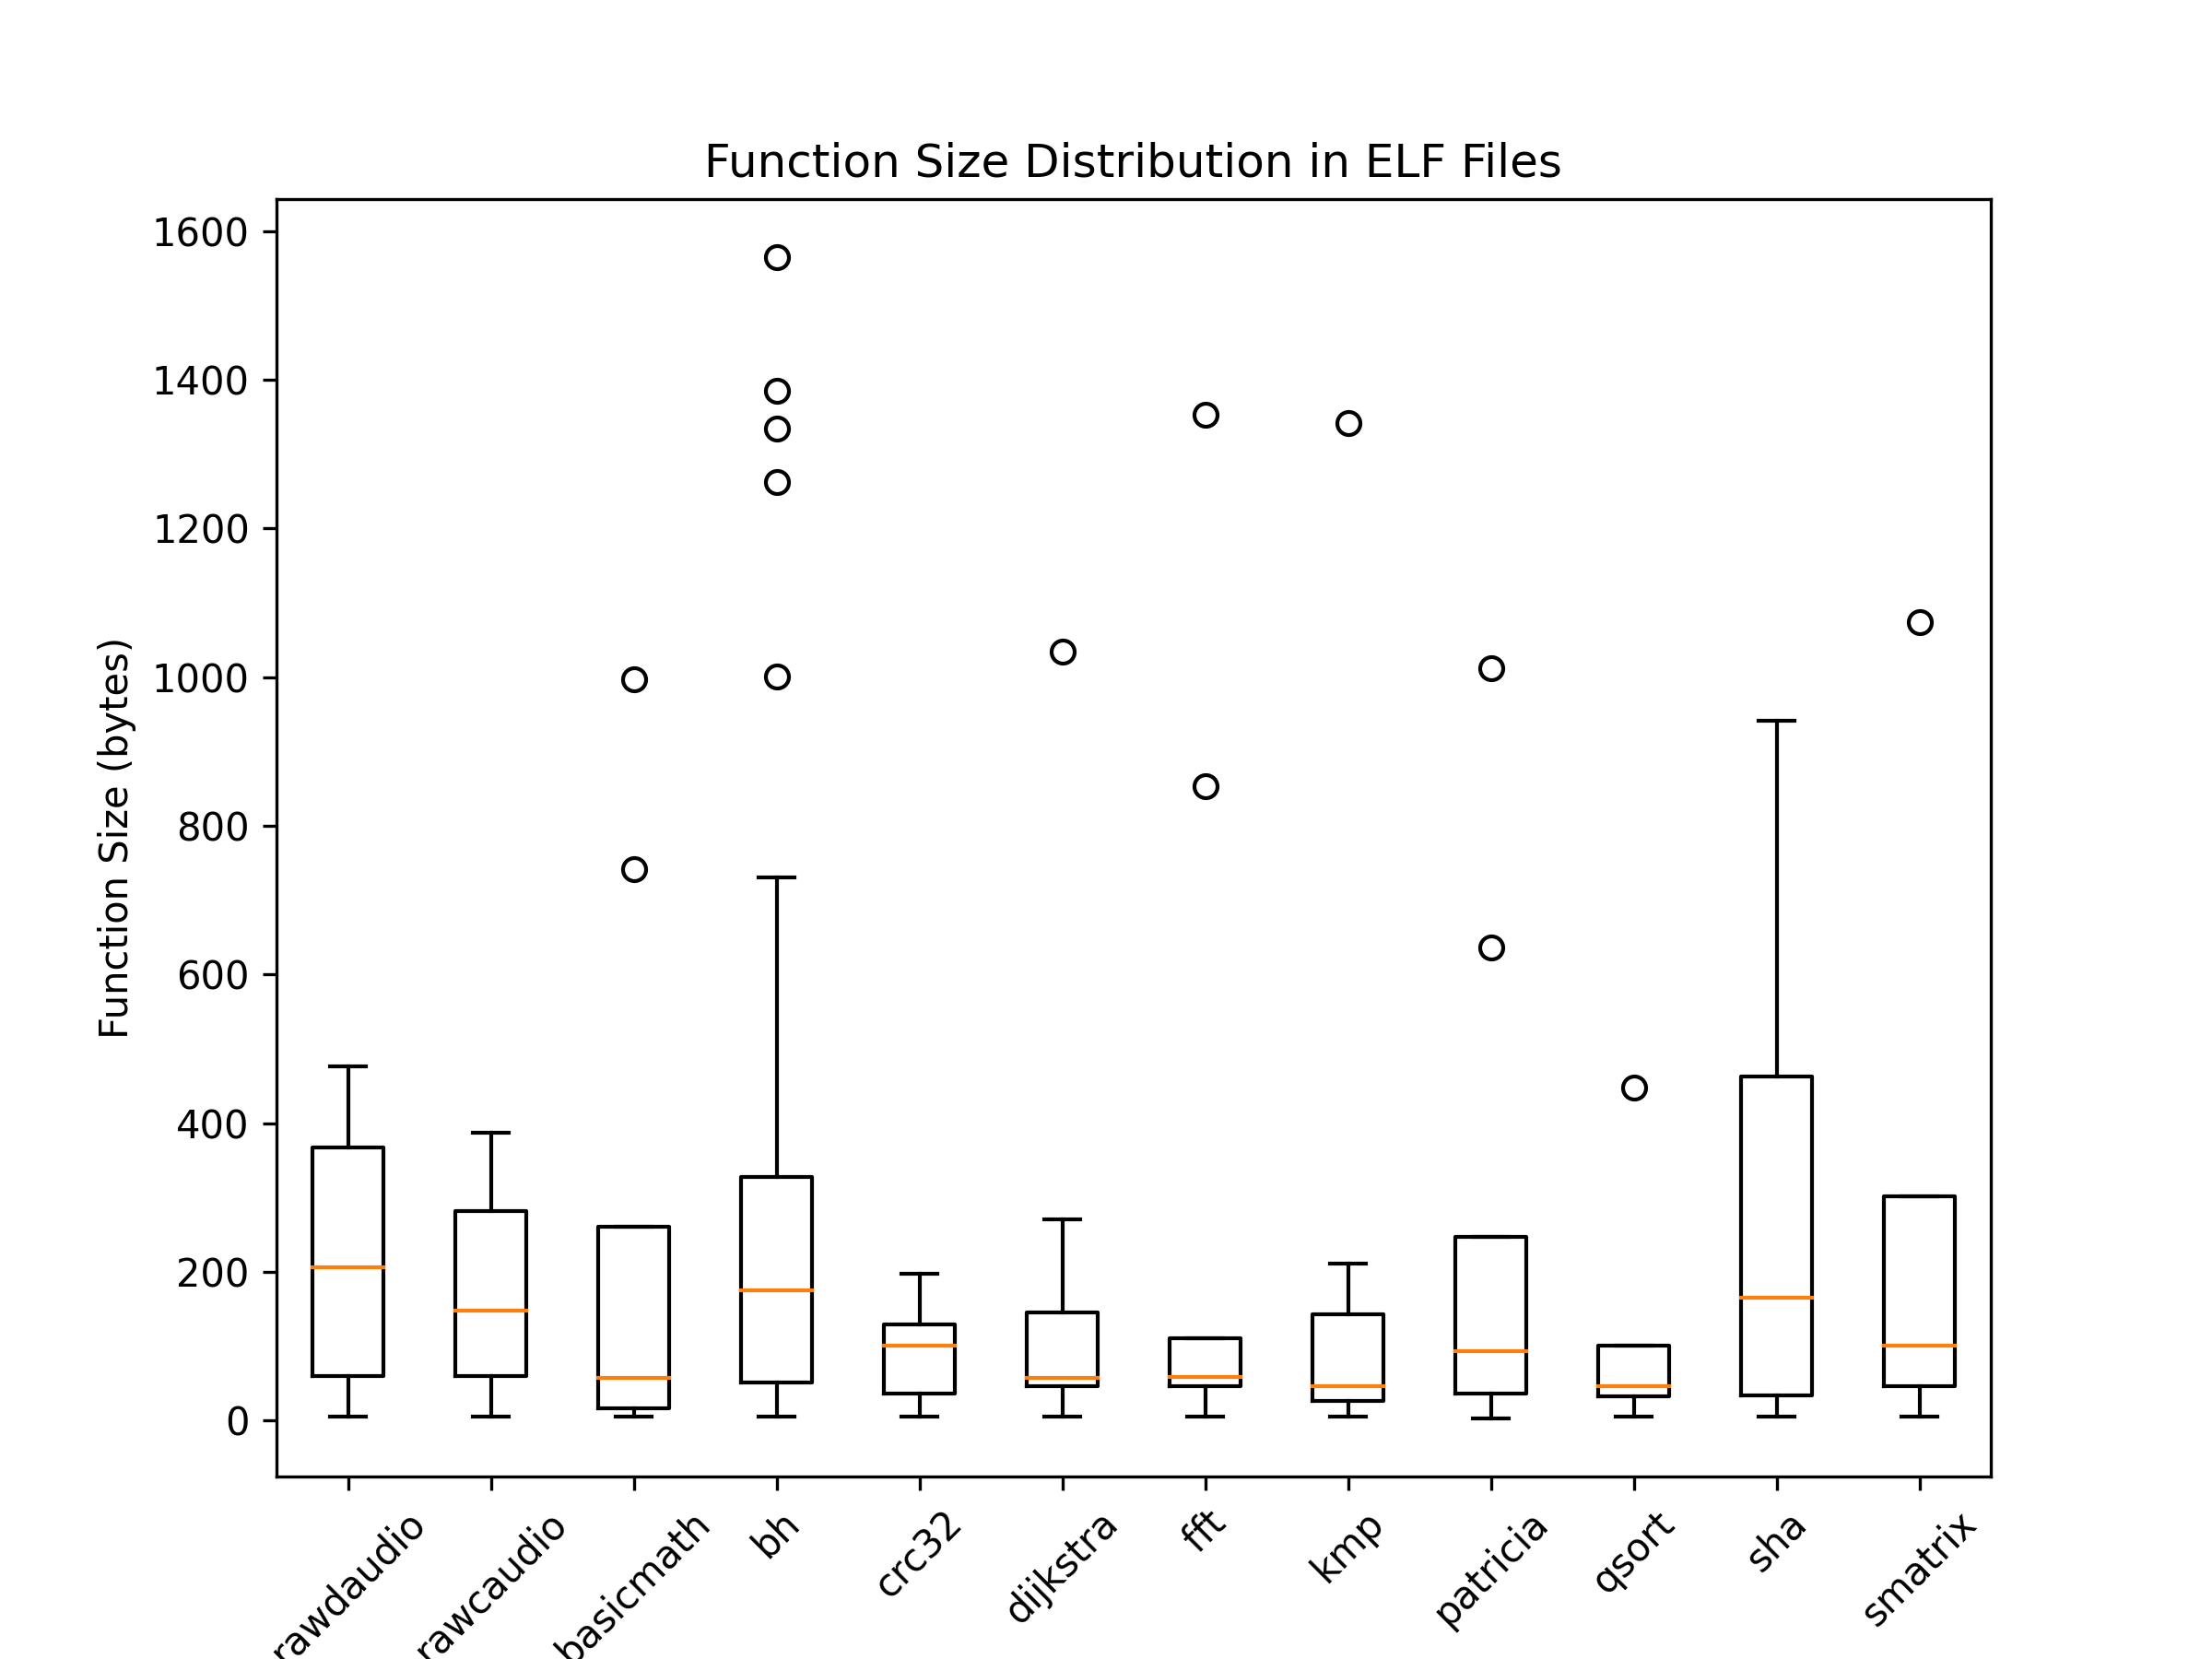
\includegraphics[width=0.9\linewidth]{Chapter-7/figs/size-profile.png}
  \caption{Per-benchmark distribution of function sizes (bytes). Each box summarizes the
           interquartile range with median (orange line); markers indicate outliers.
           Size heterogeneity explains variation in FLCR reliability improvements:
           many small functions favor higher survivability; a few large functions reduce it.}
  \label{fig:flcr-size-profile}
\end{figure}

The size distributions in Fig.~\ref{fig:flcr-size-profile} help explain cross-benchmark
differences in Fig.~\ref{fig:flcr-reliability}. Benchmarks such as those with tighter,
smaller functions tend to sustain higher success rates under growing fault density, while
benchmarks with heavy-tailed size distributions (large outliers) show earlier saturation.
This suggests two practical guidelines for FLCR deployments: (i) prioritize replication
depth for large, high-centrality functions; and (ii) ensure at least one replica of small,
frequently invoked functions to maximize aggregate reliability.

% ---------------------------------------------------
% ---------------------------------------------------
\section{Summary}
Function-Level Code Replication (FLCR) extends runtime fault tolerance by introducing
indirection at the level of function calls. Each function is validated independently,
and all invocations—direct or indirect—are redirected through the ITab or IMap to
their verified targets. This design maintains execution continuity even when individual
functions are corrupted, offering finer-grained fault isolation than region-level
replication (RLCR) under the same redundancy capacity.

However, the reliability improvement of FLCR depends strongly on the distribution of
function sizes within the program. As shown in Fig.~\ref{fig:flcr-size-profile},
benchmarks with many small, evenly sized functions exhibit much higher survivability
than those dominated by large functions. Equalizing function size across an entire
program is not straightforward, since compiler optimizations and control-flow structures
naturally produce functions of varying length and complexity.

Achieving a uniform replication granularity becomes more practical at the next level
of abstraction—\textbf{Basic-Block-Level Code Replication (BBLCR)}—where code is divided
into control-flow blocks of comparable size. BBLCR thus provides a more consistent basis
for balancing replication cost and fault coverage, extending FLCR’s principles into the
instruction path itself.